\documentclass[12pt, oneside]{article}

\usepackage[letterpaper, scale=0.89, centering]{geometry}
\usepackage{fancyhdr}
\setlength{\parindent}{0em}
\setlength{\parskip}{1em}

\pagestyle{fancy}
\fancyhf{}
\renewcommand{\headrulewidth}{0pt}
\rfoot{\href{https://creativecommons.org/licenses/by-nc-sa/2.0/}{CC BY-NC-SA 2.0} Version \today~(\thepage)}

\usepackage{amssymb,amsmath,pifont,amsfonts,comment,enumerate,enumitem}
\usepackage{currfile,xstring,hyperref,tabularx,graphicx,wasysym}
\usepackage[labelformat=empty]{caption}
\usepackage[dvipsnames,table]{xcolor}
\usepackage{multicol,multirow,array,listings,tabularx,lastpage,textcomp,booktabs}

\lstnewenvironment{algorithm}[1][] {   
    \lstset{ mathescape=true,
        frame=tB,
        numbers=left, 
        numberstyle=\tiny,
        basicstyle=\rmfamily\scriptsize, 
        keywordstyle=\color{black}\bfseries,
        keywords={,procedure, div, for, to, input, output, return, datatype, function, in, if, else, foreach, while, begin, end, }
        numbers=left,
        xleftmargin=.04\textwidth,
        #1
    }
}
{}
\lstnewenvironment{java}[1][]
{   
    \lstset{
        language=java,
        mathescape=true,
        frame=tB,
        numbers=left, 
        numberstyle=\tiny,
        basicstyle=\ttfamily\scriptsize, 
        keywordstyle=\color{black}\bfseries,
        keywords={, int, double, for, return, if, else, while, }
        numbers=left,
        xleftmargin=.04\textwidth,
        #1
    }
}
{}

\newcommand\abs[1]{\lvert~#1~\rvert}
\newcommand{\st}{\mid}

\newcommand{\A}[0]{\texttt{A}}
\newcommand{\C}[0]{\texttt{C}}
\newcommand{\G}[0]{\texttt{G}}
\newcommand{\U}[0]{\texttt{U}}

\newcommand{\cmark}{\ding{51}}
\newcommand{\xmark}{\ding{55}}

 
\begin{document}
\begin{flushright}
    \StrBefore{\currfilename}{.}
\end{flushright} \section*{Netflix intro}


What data should we encode about each Netflix account holder to help us make effective recommendations?

\vfill
\vfill

In machine learning, clustering can be used to group similar data for prediction and recommendation.  For example,
each Netflix user's viewing history can be represented as a $n$-tuple indicating their preferences about
movies in the database, where $n$ is the number of movies in the database.  People with similar tastes in movies can then be clustered to provide recommendations
of movies for one another.  Mathematically, clustering is based on a notion of distance between pairs of $n$-tuples.
 \vfill
\section*{Data types}


\begin{center}
    \begin{tabular}{p{4.6in}p{2.6in}}
    {\bf  Term} & {\bf Examples}:\\
    &  (add additional examples from class)\\
    \hline 
    {\bf set} \newline
    unordered collection of elements & $7 \in \{43, 7, 9 \}$ \qquad $2 \notin \{43, 7, 9 \}$ \\
    {\it repetition doesn't matter} & \\
    {\it Equal sets agree on membership of all elements}& \\
    \hline
    {\bf $n$-tuple} \newline
    ordered sequence of elements with $n$ ``slots" ($n >0$) & \\
    {\it repetition matters, fixed length} &\\
    {\it Equal $n$-tuples have corresponding components equal}& \\
    \hline
    {\bf string} \newline
    ordered finite sequence of elements each from specified
    set & \\
    {\it repetition matters, arbitrary finite length} &\\
    {\it Equal strings have same length and corresponding characters equal}
    \end{tabular}
\end{center}

{\it Special cases}: 

When $n=2$, the 2-tuple is called an {\bf ordered pair}.

A string of length $0$ is called the {\bf empty string} and is denoted $\lambda$.

A set with no elements is called the {\bf empty set} and is denoted $\{\}$ or $\emptyset$. \vfill
\section*{Set operations}


\fbox{\parbox{\textwidth}{To define a set we can use the roster method, set builder notation, a recursive definition, 
and also we can apply a set operation to other sets. \\

{\bf New! Cartesian product of sets} and {\bf set-wise concatenation of sets of strings}\\


{\bf Definition}: Let $X$ and $Y$ be sets.  The {\bf Cartesian product} of $X$ and $Y$, denoted
$X \times Y$, is the set of all ordered pairs $(x,y)$ where $x \in X$ and $y \in Y$
\[
X \times Y = \{ (x,y) \mid x \in X \text{ and } y \in Y \}
\]
{\bf Definition}: Let $X$ and $Y$ be sets of strings over the same alphabet. The {\bf set-wise concatenation} 
of $X$ and $Y$, denoted $X \circ Y$, is the set of all results of string concatenation $xy$ where $x \in X$ 
and $y \in Y$
\[
X \circ Y = \{ xy \mid x \in X \text{ and } y \in Y \}
\]
}}

{\bf Pro-tip}: the meaning of writing one element next to another like $xy$ depends on the data-types of $x$ and 
$y$. When $x$ and $y$ are strings, the convention is that $xy$ is the result of string concatenation. 
When $x$ and $y$ are numbers, the convention is that $xy$ is the result of multiplication. This is 
(one of the many reasons) why is it very important to declare the data-type of variables before we use them.

{\it Fill in the missing entries in the table}:

\begin{center}
\begin{tabular}{cc}
{\bf  Set} & {\bf Example elements in this set}:\\
\hline 
& \\
$B$ &\A \qquad \C \qquad \G \qquad \U \\
& \\
\hline
& \\
\phantom{$B \times B$} & $(\A, \C)$ \qquad $(\U, \U)$\\
& \\
\hline
& \\
$B \times \{-1,0,1\}$ & \\
& \\
\hline
& \\
$\{-1,0,1\} \times B$ & \\
& \\
\hline
& \\
\phantom{$\{-1,0,1\} \times \{-1,0,1\}  \times \{-1,0,1\} $} & \qquad $(0,0,0)$ \\
& \\
\hline
& \\
$ \{\A, \C, \G, \U \} \circ  \{\A, \C, \G, \U \}$& \\
& \\
\hline
& \\
\phantom{$\{G\} \circ \{G\} \circ \{G\}$} & \qquad $\G\G\G\G$ \\
& \\
\hline

\end{tabular}
\end{center}

\vfill \vfill
\section*{Defining functions}


\fbox{\parbox{\textwidth}{{\bf New! Defining functions} A function is defined by its (1) domain, 
(2) codomain, and (3) rule assigning each 
element in the domain exactly one element in the codomain.\\

The domain and codomain are nonempty sets.

The rule can be depicted as a table, formula, or English description.

The notation is 
\begin{center}
    ``Let the function FUNCTION-NAME: DOMAIN $\to$ CODOMAIN be given by \\
FUNCTION-NAME(x) = \ldots for every $x \in DOMAIN$''.
\end{center}

or 
\begin{center}
    ``Consider the function FUNCTION-NAME: DOMAIN $\to$ CODOMAIN given by \\
FUNCTION-NAME(x) = \ldots for every $x \in DOMAIN$''.
\end{center}
}}

\vfill

Example: The absolute value function 

{\bf Domain}

{\bf Codomain}

{\bf Rule}

\vfill 
 \vfill
\section*{Defining functions recursively}


When the domain of a function is a {\it recursively defined set}, the rule assigning 
images to domain elements (outputs) can also be defined recursively.

Recall: The set of RNA strands $S$ is defined (recursively) by:
\[
\begin{array}{ll}
\textrm{Basis Step: } & \A \in S, \C \in S, \U \in S, \G \in S \\
\textrm{Recursive Step: } & \textrm{If } s \in S\textrm{ and }b \in B \textrm{, then }sb \in S
\end{array}
\]
where $sb$ is string concatenation.

{\bf Definition} (Of a function, recursively) A function \textit{rnalen} that computes the length of RNA strands in $S$ is defined by:
\[
\begin{array}{llll}
& & \textit{rnalen} : S & \to \mathbb{Z}^+ \\
\textrm{Basis Step:} & \textrm{If } b \in B\textrm{ then } & \textit{rnalen}(b) & = 1 \\
\textrm{Recursive Step:} & \textrm{If } s \in S\textrm{ and }b \in B\textrm{, then  } & \textit{rnalen}(sb) & = 1 + \textit{rnalen}(s)
\end{array}
\]

The domain of \textit{rnalen} is \phantom{$S$}\\

The codomain of \textit{rnalen} is \phantom{$\mathbb{Z}^+$}\\

Example function application:
\[
rnalen(\A\C\U) = \phantom{1+ rnalen(\A\C) = 1 + (1 + rnalen(\A) ) = 1 + ( 1 + 1) = 3}
\]

\vfill

{\it Extra example}: A function \textit{basecount} that computes the number of a given base 
$b$ appearing in a RNA strand $s$ is defined recursively:
    
\[
\begin{array}{llll}
& & \textit{basecount} : S \times B & \to \mathbb{N} \\
\textrm{Basis Step:} &  \textrm{If } b_1 \in B, b_2 \in B & \textit{basecount}(~(b_1, b_2)~) & =
        \begin{cases}
            1 & \textrm{when } b_1 = b_2 \\
            0 & \textrm{when } b_1 \neq b_2 \\
        \end{cases} \\
\textrm{Recursive Step:} & \textrm{If } s \in S, b_1 \in B, b_2 \in B &\textit{basecount}(~(s b_1, b_2)~) & =
        \begin{cases}
            1 + \textit{basecount}(~(s, b_2)~) & \textrm{when } b_1 = b_2 \\
            \textit{basecount}(~(s, b_2)~) & \textrm{when } b_1 \neq b_2 \\
        \end{cases}
\end{array}
\]

$basecount(~(\A\C\U,\A)~) = basecount( ~(\A\C, \A)~) = basecount(~(\A, \A)~) = 1$\\


$basecount(~(\A\C\U,\G)~) = basecount( ~(\A\C, \G)~) = basecount(~(\A, \G)~) = 0$\\


\vfill
{\it Extra example}: The function which outputs $2^n$ when given a nonnegative integer $n$ can be defined recursively, 
because its domain is the set of nonnegative integers.

\vfill
 \vfill
\section*{Why represent numbers}


Modeling uses data-types that are 
encoded in a computer.

The details of the encoding impact the efficiency of algorithms
we use to understand the systems we are modeling and the 
impacts of these algorithms on the people using the systems.

Case study: how to encode numbers?

\phantom{
Positional representation with familiar (decimal) number encodings
\vspace{30pt}
}
\vfill \vfill
\section*{Base expansion definition}


{\bf Definition} For $b$ an integer greater than $1$ and $n$ a positive integer, 
the {\bf base $b$ expansion of $n$}  is
\[
(a_{k-1} \cdots a_1 a_0)_b
\]
where $k$ is a positive integer, $a_0, a_1, \ldots, a_{k-1}$ 
are nonnegative integers less than $b$, $a_{k-1} \neq  0$, and
\[
n =  \sum_{i=0}^{k-1} a_{i} b^{i}
\]

Notice: {\it The base $b$ expansion of a positive integer $n$ is a string over the alphabet 
$\{x \in \mathbb{N} \st x < b\}$
whose leftmost character is nonzero.}

\begin{center}
\begin{tabular}{|c|c|}
\hline
Base $b$ & Collection of possible coefficients in base $b$ expansion of  a positive integer \\
\hline
& \\
Binary ($b=2$) & $\{0,1\}$ \\
\hline
& \\
Ternary ($b=3$) & $\{0,1, 2\}$ \\
\hline
& \\
Octal ($b=8$) & $\{0,1, 2, 3, 4, 5, 6, 7\}$\\
\hline
& \\
Decimal ($b=10$) & $\{0,1, 2, 3, 4, 5, 6, 7, 8, 9\}$\\
\hline
& \\
Hexadecimal ($b=16$) &  $\{0,1, 2, 3, 4, 5, 6, 7, 8, 9, A, B, C, D, E, F\}$\\
& letter coefficient symbols represent numerical values $(A)_{16} = (10)_{10}$\\
&$(B)_{16} = (11)_{10} ~~(C)_{16} = (12)_{10} ~~
 (D)_{16} = (13)_{10} ~~ (E)_{16} = (14)_{10} ~~ (F)_{16} = (15)_{10} $\\
\hline
\end{tabular}
\end{center}

 \vfill
\section*{Base expansion examples}


\fbox{\parbox{\textwidth}{{\bf Common bases}: \hfill Binary  $b=2$ \qquad Octal $b=8$ \qquad Decimal $b=10$ \qquad Hexadecimal $b=16$
\hfill }}

{\it Examples}:

$(1401)_{2}$

\vfill

$(1401)_{10}$

\vfill
\vfill
\vfill


$(1401)_{16}$

\vfill
\vfill
\vfill
 \vfill
\section*{Algorithm definition}


\fbox{\parbox{\textwidth}{{\bf New!} An algorithm is a finite sequence of precise instructions for solving a problem.
\hfill
}} \vfill
\section*{Algorithm half}


\begin{algorithm}[caption={Algorithm for calculating integer part of half the input}]
    procedure $\textit{half}$($n$: a positive integer)
    $r$ := $0$
    while $n$ > $1$
      $r$ := $r + 1$
      $n$ := $n - 2$
    return $r$ $\{ r~\textrm{holds the result of the operation}\} $
    \end{algorithm}

 \begin{multicols}{2}
  \begin{center} 
    \begin{tabular}{c|c|c}
    $n$ & $r$  & $n > 1$?\\
    \hline 
    ~$6$~ & \phantom{~$0$~} & \phantom{~T~}\\
    \phantom{$4$} & \phantom{$1$} & \phantom{T}\\
    \phantom{$2$} & \phantom{$2$} & \phantom{T}\\
    \phantom{$0$} & \phantom{$3$} & \phantom{F}\\
    &\\
    \end{tabular}
    \end{center}
    \begin{center}
      \begin{tabular}{c|c|c}
      $n$ & $r$  & $n > 1$?\\
      \hline 
      ~$5$~ & \phantom{~$0$~} & \phantom{~T~}\\
      \phantom{$3$} & \phantom{$1$} & \phantom{T}\\
      \phantom{$1$} & \phantom{$2$} & \phantom{F}\\
      &\\
      \end{tabular}
      \end{center}    
\end{multicols}

\vfill \vfill
\section*{Algorithm log}


 \begin{algorithm}[caption={Algorithm for calculating integer part of $\log$}]
    procedure $\textit{log}$($n$: a positive integer)
    $r$ := $0$
    while $n$ > $1$
      $r$ := $r + 1$
      $n$ := $half(n)$
    return $r$ $\{ r~\textrm{holds the result of the}~\log~\textrm{operation}\} $
\end{algorithm}

\begin{multicols}{2}
  \begin{center}
    \begin{tabular}{c|c|c}
    $n$ & $r$  & $n > 1$?\\
    \hline 
    ~$8$~ & \phantom{~$0$~} & \phantom{~T~}\\
    \phantom{$4$} & \phantom{$1$} & \phantom{T}\\
    \phantom{$2$} & \phantom{$2$} & \phantom{T}\\
    \phantom{$1$} & \phantom{$3$} & \phantom{F}\\
    &\\
    \end{tabular}
    \end{center}
  \begin{center}
    \begin{tabular}{c|c|c}
    $n$ & $r$  & $n > 1$?\\
    \hline 
    ~$6$~ & \phantom{~$0$~} & \phantom{~T~}\\
    \phantom{$3$} & \phantom{$1$} & \phantom{T}\\
    \phantom{$1$} & \phantom{$2$} & \phantom{F}\\
    &\\
    \end{tabular}
    \end{center}
\end{multicols}

\vfill

\fbox{\parbox{\textwidth}{
$2^0 = 1$~~\hfill $2^1=2$~~\hfill $2^2=4$~~\hfill $2^3=8$~~
\hfill $2^4=16$~~\hfill $2^5=32$~~
\hfill $2^6=64$~~\hfill $2^7=128$~~
\hfill $2^8=256$~~\hfill $2^9=512$~~
\hfill $2^{10}=1024$}} \vfill
\section*{Division algorithm}


{\bf Integer division and remainders} (aka The Division Algorithm) Let $n$ be an integer 
and $d$ a positive integer. There are unique integers $q$ and $r$, with $0 \leq r < d$, such that 
$n = dq + r$. In this case, $d$ is called the divisor, $n$ is called the dividend, 
$q$ is called the quotient, 
and $r$ is called the remainder. We write $q=n \textbf{ div } d$ and $r=n \textbf{ mod } d$.

\textit{Extra example}: How do $\textbf{ div }$ and $\textbf{ mod }$ compare to $/$ and $\%$ in Java and python?

\vfill
 \vfill
\section*{Base expansion algorithms}


{\bf Two algorithms for constructing base $b$ expansion from decimal representation}

{\bf Most significant first}: Start with left-most coefficient of expansion
\begin{multicols}{2}
\begin{algorithm}[caption={Calculating integer part of $\log_b$}]
procedure $\textit{logb}$($n, b$: positive integers with $b > 1$)
$r$ := $0$
while $n$ > $1$
  $r$ := $r + 1$
  $n$ := $n$ div $b$
return $r$ $\{ r~\textrm{holds the result of the}~\log_b~\textrm{operation}\}$
\end{algorithm}
\columnbreak
\begin{algorithm}[caption={Calculating base $b$ expansion, from left}]
procedure $\textit{baseb1}$($n, b$: positive integers with $b > 1$)
$v$ := $n$
$k$ := $logb(n,b) + 1$
for $i$ := $1$ to $k$
  $a_{k-i}$ := $0$
  while $v \geq b^{k-i}$
    $a_{k-i}$ := $a_{k-i} + 1$
    $v$ := $v -  b^{k-i}$
return $(a_{k-1}, \ldots, a_0) \{(a_{k-1} \ldots a_0)_b~\textrm{ is the base } b \textrm{ expansion of } n \}$
\end{algorithm}
\end{multicols}

\vfill
\vfill

{\bf Least significant first}: Start with right-most coefficient of expansion

\begin{multicols}{2}
  \begin{minipage}{3.2in}
    Idea: {\tiny(when $k > 1$)} 
    \begin{align*}
      n &= a_{k-1} b^{k-1} + \cdots + a_1 b + a_0 \\
        &= b ( a_{k-1} b^{k-2} + \cdots + a_1) + a_0\end{align*}
    so $a_0 = n \textbf{ mod } b$ and $a_{k-1} b^{k-2} + \cdots + a_1 = n \textbf{ div } b$.

\end{minipage}
\columnbreak
\begin{algorithm}[caption={Calculating base $b$ expansion, from right}]
procedure $\textit{baseb2}$($n, b$: positive integers with $b > 1$)
$q$ := $n$
$k$ := $0$
while $q  \neq 0$
  $a_{k}$ := $q$ mod $b$
  $q$ := $q$ div $b$
  $k$ := $k+1$
return $(a_{k-1}, \ldots, a_0) \{(a_{k-1} \ldots a_0)_b~\textrm{ is the base } b \textrm{ expansion of } n \}$
\end{algorithm}
\end{multicols}

\vfill
\vfill \vfill
\section*{Base expansion review}


Find and fix any and all mistakes with the following:
\begin{itemize}
\item[(a)] $(1)_2 = (1)_8$
\item[(b)] $(142)_{10} = (142)_{16}$
\item[(c)] $(20)_{10} = (10100)_2$
\item[(d)] $(35)_8 = (1D)_{16}$
\end{itemize} \vfill
\section*{Base conversion algorithm}


{\it Recall the definition of base expansion we discussed:}



{\bf Definition} For $b$ an integer greater than $1$ and $n$ a positive integer, 
the {\bf base $b$ expansion of $n$}  is
\[
(a_{k-1} \cdots a_1 a_0)_b
\]
where $k$ is a positive integer, $a_0, a_1, \ldots, a_{k-1}$ 
are nonnegative integers less than $b$, $a_{k-1} \neq  0$, and
\[
n =  \sum_{i=0}^{k-1} a_{i} b^{i}
\]

Notice: {\it The base $b$ expansion of a positive integer $n$ is a string over the alphabet 
$\{x \in \mathbb{N} \st x < b\}$
whose leftmost character is nonzero.}

\begin{center}
\begin{tabular}{|c|c|}
\hline
Base $b$ & Collection of possible coefficients in base $b$ expansion of  a positive integer \\
\hline
& \\
Binary ($b=2$) & $\{0,1\}$ \\
\hline
& \\
Ternary ($b=3$) & $\{0,1, 2\}$ \\
\hline
& \\
Octal ($b=8$) & $\{0,1, 2, 3, 4, 5, 6, 7\}$\\
\hline
& \\
Decimal ($b=10$) & $\{0,1, 2, 3, 4, 5, 6, 7, 8, 9\}$\\
\hline
& \\
Hexadecimal ($b=16$) &  $\{0,1, 2, 3, 4, 5, 6, 7, 8, 9, A, B, C, D, E, F\}$\\
& letter coefficient symbols represent numerical values $(A)_{16} = (10)_{10}$\\
&$(B)_{16} = (11)_{10} ~~(C)_{16} = (12)_{10} ~~
 (D)_{16} = (13)_{10} ~~ (E)_{16} = (14)_{10} ~~ (F)_{16} = (15)_{10} $\\
\hline
\end{tabular}
\end{center}

 
We write an algorithm for converting from base $b_1$ expansion to base $b_2$ expansion:

\phantom{
Earlier, we saw (two different) algorithms for, given 
a target base $b$, converting from decimal to base $b$ expansions. 
We will use either one of these as a subroutine in this algorithm.\\
Given a base expansion in base $b_1$:\\
Step 1: Use the definition of base expansion to calculate the value of
    this number (in decimal).\\
Step 2: Use the Least Significant First algorithm to write this value in 
    base $b_2$ and output the result.
}
\vspace{200pt} \vfill
\section*{Fixed width definition}


{\bf Definition} For $b$ an integer greater than $1$, $w$ a positive integer, 
and $n$ a nonnegative integer
$\underline{\phantom{\hspace{1in}}}$, ~
the {\bf base $b$ fixed-width $w$ expansion of $n$}  is
\[
(a_{w-1} \cdots a_1 a_0)_{b,w}
\]
where  $a_0, a_1, \ldots, a_{w-1}$ are nonnegative integers less than $b$ and
\[
n =  \sum_{i=0}^{w-1} a_{i} b^{i}
\]
 \vfill
\section*{Fixed width example}


\begin{center}
    \begin{tabular}{|c|c|c|c|c|}
    \hline
    Decimal &  Binary  & Binary fixed-width $10$& Binary fixed-width $7$ & Binary fixed-width $4$\\
    $b=10$ & $b=2$ & $b=2$, $w =  10$& $b=2$, $w =  7$& $b=2$, $w =  4$ \\
    \hline 
    &&&&  \\
    $(20)_{10}$&\phantom{$(10100)_{2}$\qquad\qquad}&&  &\\
    &&&&  \\
    &(a)&(b)&(c)&(d)  \\
    \hline
    \end{tabular}
    \end{center}
 \vfill
\section*{Fixed width fractional definition}


{\bf Definition} For $b$ an integer greater than $1$, $w$ a positive integer, 
$w'$ a positive  integer, and $x$ a real number the {\bf base $b$ fixed-width 
expansion of $x$ with integer part width $w$  and fractional part width $w'$} is
$(a_{w-1} \cdots a_1 a_0 .  c_{1} \cdots c_{w'})_{b,w,w'}$
where  $a_0, a_1, \ldots, a_{w-1}, c_1, \ldots, c_{w'}$ are nonnegative integers less than $b$ and
$$x \geq \sum_{i=0}^{w-1} a_{i} b^{i} + \sum_{j=1}^{w'}  c_{j} b^{-j} \hfill
\textrm{\qquad and \qquad}
\hfill x < \sum_{i=0}^{w-1} a_{i} b^{i} + \sum_{j=1}^{w'} c_{j} b^{-j} + b^{-w'}$$

\begin{center}
\begin{tabular}{|c|p{5in}|}
\hline
& \\
$3.75$  in fixed-width binary,& \\
integer part width $2$,&\\
 fractional part width $8$ & \\
& \\
\hline
& \\
$0.1$  in fixed-width binary, & \\
integer part width $2$, &\\
 fractional part width $8$ & \\
& \\
\hline
\end{tabular}
\end{center}

\includegraphics[width=2in]{../../resources/images/ArithmeticDemo.png}

Note: Java uses floating point, not fixed width representation, but similar rounding errors appear in both.
 \vfill
\section*{Expansion summary}


\begin{center}
    \begin{tabular}{|p{3.7in}|p{3.7in}|}
    \hline 
    &   \\
    {\bf base $b$ expansion of $n$}  & {\bf base $b$ fixed-width $w$ expansion of $n$}  \\
    & \\
    \hline  
    For $b$ an integer greater than $1$ and $n$ a positive integer, 
    the {\bf base $b$ expansion of $n$}  is $(a_{k-1} \cdots a_1 a_0)_b$
    where $k$ is a positive integer, $a_0, a_1, \ldots, a_{k-1}$ are nonnegative integers 
    less than $b$, $a_{k-1} \neq  0$, and $n =  a_{k-1} b^{k-1} + \cdots + a_1b + a_0$
    & 
    For $b$ an integer greater than $1$, $w$ a positive integer, and $n$ a nonnegative integer
    with $n <  b^w$, the {\bf base $b$ fixed-width $w$ expansion of $n$}  is
    $(a_{w-1} \cdots a_1 a_0)_{b,w}$
    where  $a_0, a_1, \ldots, a_{w-1}$ are nonnegative integers less than $b$ and 
    $n =  a_{w-1} b^{w-1} + \cdots + a_1b + a_0$\\
    \hline
    \end{tabular}
\end{center} \vfill
\section*{Negative int expansions}


{\bf Representing negative integers in binary}: Fix a positive integer  width for the representation  $w$, $w >1$.

\begin{tabular}{|cc|p{3.4in}|p{3.7in}|}
\hline
& & To  represent a positive integer $n$ & To represent a negative integer $-n$\\
\hline
&& &  \\
&\parbox[t]{2mm}{\multirow{4}{*}{\rotatebox[origin=c]{90}{Sign-magnitude}}} &
$[ 0a_{w-2} \cdots a_0]_{s,w}$, where $n =  (a_{w-2} \cdots a_0)_{2,w-1}$& 
$[1a_{w-2} \cdots a_0]_{s,w}$
, where $n =  (a_{w-2} \cdots a_0)_{2,w-1}$\\
&& & \\
&& Example $n=17$, $w=7$:  & Example $-n=-17$, $w=7$: \\
&& & \\
&& & \\
&& & \\
&& & \\
&& & \\
&& & \\
&& & \\
\hline
&&  &  \\
&\parbox[t]{2mm}{\multirow{4}{*}{\rotatebox[origin=c]{90}{2s complement}}} &
$[0a_{w-2} \cdots a_0]_{2c,w}$, where $n =  (a_{w-2} \cdots a_0)_{2,w-1}$& $[1a_{w-2} \cdots a_0]_{2c,w}$, where $2^{w-1} - n =  (a_{w-2} \cdots a_0)_{2,w-1}$\\
&& & \\
&& Example $n=17$, $w=7$:  & Example $-n=-17$, $w=7$: \\
&& & \\
&& & \\
&& & \\
&& & \\
&& & \\
&& & \\
&& & \\
\hline
&&  &  \\
\parbox[t]{1.5mm}{\multirow{4}{*}{\rotatebox[origin=c]{90}{{\it Extra example:}}}} 
& \parbox[t]{2mm}{\multirow{4}{*}{\rotatebox[origin=c]{90}{1s complement}}} &
$[0a_{w-2} \cdots a_0]_{1c,w}$, where $n =  (a_{w-2} \cdots a_0)_{2,w-1}$& $[1\bar{a}_{w-2} \cdots \bar{a}_0]_{1c,w}$, where $n =  (a_{w-2} \cdots a_0)_{2,w-1}$ and we define  $\bar{0} = 1$ and $\bar{1} = 0$.\\
&& & \\
&& Example $n=17$, $w=7$:  & Example $-n=-17$, $w=7$: \\
&& & \\
&& & \\
&& & \\
&& & \\
&& & \\
\hline
\end{tabular} \vfill
\section*{Calculating 2s complement}


For positive integer $n$, to represent $-n$ in 
$2$s complement with width $w$,
\begin{itemize}
    \item Calculate $2^{w-1} - n$, convert 
    result to binary fixed-width $w-1$, pad 
    with leading $1$, or
    \item Express $-n$ as a sum of powers of $2$, 
    where the leftmost $2^{w-1}$ is negative weight, or
    \item Convert $n$ to binary fixed-width, 
    flip bits, add 1 (ignore overflow)
\end{itemize}

{\it Challenge: use definitions to explain why
each of these approaches works.} \vfill
\section*{Representing zero}


{\bf Representing $0$}:

So far, the definitions of base expansions treat
positive and negative integers. What about $0$?

\begin{tabular}{|cc|p{3.4in}|p{3.7in}|}
   \hline
   & & To  represent a {\bf non-negative} integer $n$ & To represent a {\bf non-positive} integer $-n$\\
   \hline
   && &  \\
   &\parbox[t]{2mm}{\multirow{4}{*}{\rotatebox[origin=c]{90}{Sign-magnitude}}} &
   $[ 0a_{w-2} \cdots a_0]_{s,w}$, where $n =  (a_{w-2} \cdots a_0)_{2,w-1}$& 
   $[1a_{w-2} \cdots a_0]_{s,w}$
   , where $n =  (a_{w-2} \cdots a_0)_{2,w-1}$\\
   && & \\
   && Example $n=0$, $w=7$:  & Example $-n=0$, $w=7$: \\
   && & \\
   && & \\
   && & \\
   && & \\
   && & \\
   && (a) & (b)\\
   \hline
   &&  &  \\
   &\parbox[t]{2mm}{\multirow{4}{*}{\rotatebox[origin=c]{90}{2s complement}}} &
   $[0a_{w-2} \cdots a_0]_{2c,w}$, where $n =  (a_{w-2} \cdots a_0)_{2,w-1}$& $[1a_{w-2} \cdots a_0]_{2c,w}$, where $2^{w-1} - n =  (a_{w-2} \cdots a_0)_{2,w-1}$\\
   && & \\
   && Example $n=0$, $w=7$:  & Example $-n=0$, $w=7$: \\
   && & \\
   && & \\
   && & \\
   && & \\
   && & \\
   && (c) & (d) \\
   \hline
\end{tabular} \vfill
\section*{Fixed width addition}


{\bf Fixed-width addition}: adding one bit at time, using the usual column-by-column and carry arithmetic, and dropping the carry from the leftmost column so the result is the same width as the summands.  {\it Does this give the right value for the sum?}
\begin{multicols}{3}
\begin{align*}
   & (1~ 1~ 0~ 1~ 0~ 0)_{2,6}\\
+ & (0~ 0~ 0~ 1~ 0~ 1)_{2,6}\\
&\overline{\phantom{(1~1~1~0~0~1)_{2,6}}}\\
\end{align*}

\begin{align*}
   & [1~ 1~ 0~ 1~ 0~ 0]_{s,6}\\
+ & [0~ 0~ 0~ 1~ 0~ 1]_{s,6}\\
&\overline{\phantom{(1~1~1~0~0~1)_2}}\\
\end{align*}

\begin{align*}
   & [1~ 1~ 0~ 1~ 0~ 0]_{2c,6}\\
+ & [0~ 0~ 0~ 1~ 0~ 1]_{2c,6}\\
&\overline{\phantom{(1~1~1~0~0~1)_2}}\\
\end{align*}
\end{multicols} \vfill
\section*{Circuits basics}


In a {\bf combinatorial circuit} (also known as
a {\bf logic circuit}), we have {\bf logic gates} 
connected
by {\bf wires}. The inputs to the circuits are the 
values set on the input wires: possible
values are 0 (low) or 1 (high). The values
flow along the wires from left to right.
A wire may be split into two or more wires, 
indicated with a filled-in circle (representing
solder). Values stay the same along a wire. When 
one or more wires flow into a gate, the output 
value of that gate is computed
from the input values based on the gate's definition
table. Outputs of gates may become inputs to other
gates.  \vfill
\section*{Logic gates definitions}


\begin{multicols}{2}
\begin{center}\begin{tabular}{cc|c}
Inputs &  & Output \\
$x$ & $y$ & $x \text{ AND } y$  \\
\hline
$1$ & $1$ & $1$\\
$1$ & $0$ & $0$\\
$0$ & $1$ & $0$\\
$0$ & $0$ & $0$\\
\end{tabular}\end{center}
\columnbreak
\begin{center}\includegraphics[height=0.6in]{../../resources/images/xANDy.png} \end{center}
\end{multicols}

\begin{multicols}{2}
\begin{center}\begin{tabular}{cc|c}
Inputs &  & Output \\
$x$ & $y$ & $x \text{ XOR } y$  \\
\hline
$1$ & $1$ & $0$\\
$1$ & $0$ & $1$\\
$0$ & $1$ & $1$\\
$0$ & $0$ & $0$\\
\end{tabular}\end{center}
\columnbreak
\begin{center}\includegraphics[height=0.4in]{../../resources/images/xXORy.png} \end{center}
\end{multicols}

\begin{multicols}{2}
\begin{center}\begin{tabular}{c|c}
Input  & Output \\
$x$ & $\text{NOT } x$  \\
\hline
$1$ & $0$\\
$0$ & $1$\\
\end{tabular}\end{center}
\columnbreak
\begin{center}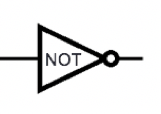
\includegraphics[height=0.5in]{../../resources/images/NOTx.png} \end{center}
\end{multicols}

%
 \vfill
\section*{Digital circuits basic examples}


{\bf Example digital circuit}: 

\begin{multicols}{2}
\begin{center}
   \includegraphics[width=1.2in]{../../resources/images/circuitEx.png} 
\end{center}
\columnbreak
Output when $x=1, y=0, z=0, w = 1$ is \underline{\phantom{$~~~0~~~$}}
Output when $x=1, y=1, z=1, w = 1$ is \underline{\phantom{$~~~0~~~$}}
Output when $x=0, y=0, z=0, w = 1$ is \underline{\phantom{$~~~0~~~$}}
\phantom{Output when $x=0, y=0, z=0, w = 0$ is \underline{\phantom{$~~~0~~~$}}}
\end{multicols}



Draw a logic circuit with inputs $x$ and $y$ whose output  is always $0$.  {\it  Can you use exactly 1 gate?}


\vspace{40pt} \vfill
\section*{Half adder circuit}


{\bf Fixed-width addition}: adding one bit at time, using the usual column-by-column and carry arithmetic, and dropping the carry from the leftmost column so the result is the same width as the summands.  In many cases, this gives representation of the correct value for the sum when we interpret the summands
in fixed-width binary or in 2s complement.

For single column:
\begin{center}
\begin{tabular}{cc|cc}
\multicolumn{2}{c|}{Input}  & \multicolumn{2}{|c}{Output}  \\
$x_0$ & $y_0$ & $c_0$ & $s_0$  \\
\hline
$1$ & $1$ & \phantom{$1$} & \phantom{$0$} \\
$1$ & $0$ & \phantom{$0$} & \phantom{$1$}\\
$0$ & $1$ & \phantom{$0$} & \phantom{$1$}\\
$0$ & $0$ & \phantom{$0$} & \phantom{$0$}\\
\end{tabular}
\end{center}

\begin{center}
\includegraphics[width=1.5in]{../../resources/images/half-adder.png}
\end{center} \vfill
\section*{Two bit adder circuit}


Draw a logic circuit that implements fixed-width 2 binary addition:
\begin{itemize}
\item Inputs  $x_0, y_0, x_1, y_1$ represent $(x_1  x_0)_{2,2}$ and $(y_1 y_0)_{2,2}$
\item Outputs  $z_0, z_1, z_2$ represent $(z_2  z_1 z_0)_{2,3} = (x_1  x_0)_{2,2} + (y_1 y_0)_{2,2}$ (may require up to width  $3$)
\end{itemize}

{\it First approach}: half-adder for each column, then combine carry from right column with sum of left column


Write expressions for the circuit output values in terms of input values:

$z_0 = \underline{\phantom{x_0 \oplus y_0\hspace{3in}}}$

$z_1 = \underline{\phantom{(x_1 \oplus y_1) \oplus c_0}\hspace{2.5in}}$ \phantom{where $c_0 = x_0 \land y_0$}

$z_2 = \underline{\phantom{(c_0 \land (x_1 \oplus y_1)) \oplus c_1}\hspace{2in}}$ \phantom{where $c_1 = x_1 \land y_1$}\\

\includegraphics[width=1.7in]{../../resources/images/width-2-adder.png}



{\it Second approach}: for middle column, first add carry from right column to $x_1$, then add result to $y_1$


Write expressions for the circuit output values in terms of input values:

$z_0 = \underline{\phantom{x_0 \oplus y_0}\hspace{3in}}$

$z_1 = \underline{ \phantom{(c_0 \oplus x_1) \oplus y_1}\hspace{2.4in}}$ \phantom{where $c_0 = x_0 \land y_0$}

$z_2 = \underline{\phantom{(c_0 \land x_1) \oplus ((c_0 \oplus x_1)\land y_1)}\hspace{1.5in}}$

\vfill

{\it Extra example} Describe how to generalize this addition circuit for larger width inputs.

 \vfill
\end{document}